\chapter{MapReduce Basics}
\label{chapter2}

The only feasible approach to tackling large-data problems today is to
divide and conquer, a fundamental concept in computer science that is
introduced very early in typical undergraduate curricula.  The basic
idea is to partition a large problem into smaller sub-problems.  To
the extent that the sub-problems are independent~\cite{Amdahl_1967},
they can be tackled in parallel by different workers---threads in a
processor core, cores in a multi-core processor, multiple processors
in a machine, or many machines in a cluster.  Intermediate results
from each individual worker are then combined to yield the final
output.\footnote{We note that promising technologies such as quantum
or biological computing could potentially induce a paradigm shift, but
they are far from being sufficiently mature to solve real world
problems.}

The general principles behind divide-and-conquer algorithms are
broadly applicable to a wide range of problems in many different
application domains.  However, the details of their implementations
are varied and complex.  For example, the following are just some of
the issues that need to be addressed:

\begin{itemize}

\item How do we break up a large problem into smaller tasks?  
  More specifically, how do we decompose the problem so that the
  smaller tasks can be executed in parallel?

\item How do we assign tasks to workers distributed across a
  potentially large number of machines (while keeping in mind that
  some workers are better suited to running some tasks than others,
  e.g., due to available resources, locality constraints, etc.)?

\item How do we ensure that the workers get the data they need?

\item How do we coordinate synchronization among the different
  workers?

\item How do we share partial results from one worker that is needed
  by another?

\item How do we accomplish all of the above in the face of software
  errors and hardware faults?

\end{itemize}

In traditional parallel or distributed programming environments, the
developer needs to explicitly address many (and sometimes, all) of the
above issues.  In shared memory programming, the developer needs to
explicitly coordinate access to shared data structures through
synchronization primitives such as mutexes, to explicitly handle
process synchronization through devices such as barriers, and to
remain ever vigilant for common problems such as deadlocks and race
conditions.  Language extensions, like OpenMP for shared memory
parallelism,\footnote{\texttt{http://www.openmp.org/}} or libraries
implementing the Message Passing Interface (MPI) for cluster-level
parallelism,\footnote{\texttt{http://www.mcs.anl.gov/mpi/}} provide logical
abstractions that hide details of operating system synchronization and
communications primitives.  However, even with these extensions,
developers are still burdened to keep track of how resources are made
available to workers.  Additionally, these frameworks are mostly
designed to tackle processor-intensive problems and have only
rudimentary support for dealing with very large amounts of input data.
When using existing parallel computing approaches for large-data
computation, the programmer must devote a significant amount of
attention to low-level system details, which detracts from
higher-level problem solving.

One of the most significant advantages of MapReduce is that it
provides an abstraction that hides many system-level details from the
programmer.  Therefore, a developer can focus on what computations
need to be performed, as opposed to how those computations are
actually carried out or how to get the data to the processes that
depend on them.  Like OpenMP and MPI, MapReduce provides a means to
distribute computation without burdening the programmer with the
details of distributed computing (but at a different level of
granularity).  However, organizing and coordinating large amounts of
computation is only part of the challenge.  Large-data processing by
definition requires bringing data and code together for computation to
occur---no small feat for datasets that are terabytes and perhaps
petabytes in size!  MapReduce addresses this challenge by providing a
simple abstraction for the developer, transparently handling most of
the details behind the scenes in a scalable, robust, and efficient
manner.  As we mentioned in Chapter~\ref{chapter1}, instead of moving
large amounts of data around, it is far more efficient, if possible,
to move the code to the data.  This is operationally realized by
spreading data across the local disks of nodes in a cluster and
running processes on nodes that hold the data.  The complex task of
managing storage in such a processing environment is typically handled
by a distributed file system that sits underneath MapReduce.

This chapter introduces the MapReduce programming model and the
underlying distributed file system.  We start in
Section~\ref{chapter2:functional} with an overview of functional
programming, from which MapReduce draws its inspiration.
Section~\ref{chapter2:mappers-and-reducers} introduces the basic
programming model, focusing on mappers and reducers.
Section~\ref{chapter2:execution-framework} discusses the role of the
execution framework in actually running MapReduce programs (called
jobs).  Section~\ref{chapter2:partitioners-and-combiners} fills in
additional details by introducing partitioners and combiners, which
provide greater control over data flow.  MapReduce would not be
practical without a tightly-integrated distributed file system that
manages the data being processed; Section~\ref{chapter2:dfs} covers
this in detail.  Tying everything together, a complete cluster
architecture is described in
Section~\ref{chapter2:cluster-architecture} before the chapter ends
with a summary.

\section{Functional Programming Roots}
\label{chapter2:functional}

MapReduce has its roots in functional programming, which is
exemplified in languages such as Lisp and ML.\footnote{However, there
are important characteristics of MapReduce that make it non-functional
in nature---this will become apparent later.} A key feature of
functional languages is the concept of higher-order functions, or
functions that can accept other functions as arguments.  Two common
built-in higher order functions are \emph{map} and \emph{fold},
illustrated in Figure~\ref{figure:chapter2:functional}.  Given a list,
\emph{map} takes as an argument a function $f$ (that takes a single
argument) and applies it to all elements in a list (the top part of
the diagram).  Given a list, \emph{fold} takes as arguments a function
$g$ (that takes two arguments) and an initial value:\ $g$ is first
applied to the initial value and the first item in the list, the
result of which is stored in an intermediate variable.  This
intermediate variable and the next item in the list serve as the
arguments to a second application of $g$, the results of which are
stored in the intermediate variable.  This process repeats until all
items in the list have been consumed; \emph{fold} then returns the
final value of the intermediate variable.  Typically, \emph{map} and
\emph{fold} are used in combination.  For example, to compute the sum
of squares of a list of integers, one could map a function that
squares its argument (i.e., $\lambda x. x^2$) over the input list, and
then fold the resulting list with the addition function (more
precisely, $\lambda x \lambda y. x + y$) using an initial value of
zero.

\begin{figure}[t]
\begin{center}
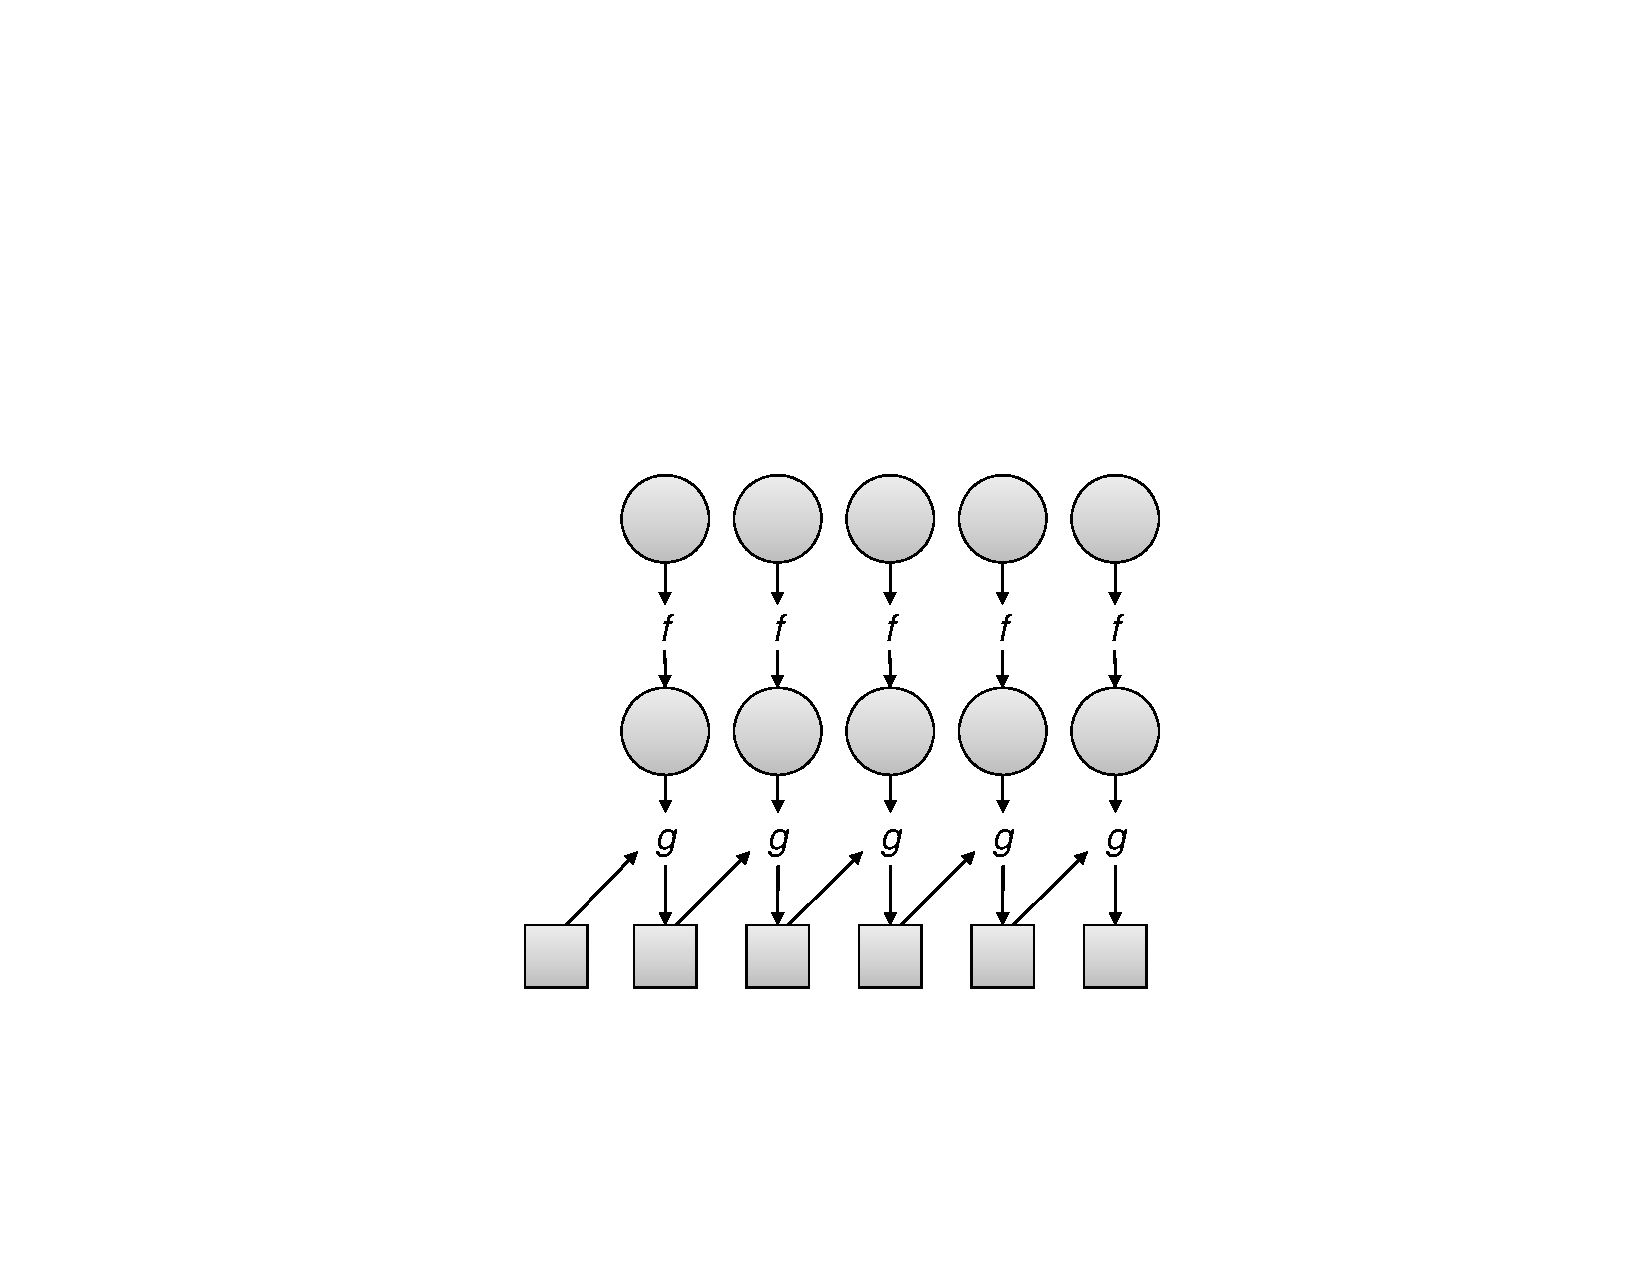
\includegraphics[scale=0.6]{figures/fig-ch2-functional-programming.pdf}
\end{center}
\caption{Illustration of \emph{map} and \emph{fold}, two higher-order
  functions commonly used together in functional programming:\ \emph{
    map} takes a function $f$ and applies it to every element in a
    list, while \emph{fold} iteratively applies a function $g$ to
    aggregate results.}
\label{figure:chapter2:functional}
\end{figure}

We can view \emph{map} as a concise way to represent the transformation
of a dataset (as defined by the function $f$).  In the same vein, we
can view \emph{fold} as an aggregation operation, as defined by the
function $g$.  One immediate observation is that the application of
$f$ to each item in a list (or more generally, to elements in a large
dataset) can be parallelized in a straightforward manner, since each
functional application happens in isolation.  In a cluster, these
operations can be distributed across many different machines.  The
\emph{fold} operation, on the other hand, has more restrictions on data
locality---elements in the list must be ``brought together'' before
the function $g$ can be applied.  However, many real-world
applications do not require $g$ to be applied to \emph{all} elements of
the list.  To the extent that elements in the list can be divided into
groups, the fold aggregations can also proceed in parallel.
Furthermore, for operations that are commutative and associative,
significant efficiencies can be gained in the \emph{fold} operation
through local aggregation and appropriate reordering.

In a nutshell, we have described MapReduce.  The map phase in
MapReduce roughly corresponds to the \emph{map} operation in functional
programming, whereas the reduce phase in MapReduce roughly corresponds
to the \emph{fold} operation in functional programming.  As we will
discuss in detail shortly, the MapReduce execution framework
coordinates the map and reduce phases of processing over large amounts
of data on large clusters of commodity machines.

Viewed from a slightly different angle, MapReduce codifies a generic
``recipe'' for processing large datasets that consists of two stages.
In the first stage, a user-specified computation is applied over all
input records in a dataset.  These operations occur in parallel and
yield intermediate output that is then aggregated by another
user-specified computation.  The programmer defines these two types of
computations, and the execution framework coordinates the actual
processing (very loosely, MapReduce provides a functional
abstraction).  Although such a two-stage processing structure may
appear to be very restrictive, many interesting algorithms can be
expressed quite concisely---especially if one decomposes complex
algorithms into a sequence of MapReduce jobs.  Subsequent chapters in
this book focus on how a number of algorithms can be implemented in
MapReduce.

To be precise, MapReduce can refer to three distinct but related
concepts.  First, MapReduce is a programming model, which is the sense
discussed above.  Second, MapReduce can refer to the execution
framework (i.e., the ``runtime'') that coordinates the execution of
programs written in this particular style.  Finally, MapReduce can
refer to the software implementation of the programming model and the
execution framework:\ for example, Google's proprietary implementation
vs.\ the open-source Hadoop implementation in Java.  And in fact,
there are many implementations of MapReduce, e.g., targeted
specifically for multi-core processors~\cite{Ranger_etal_2007}, for
GPGPUs~\cite{HeB_etal_2008}, for the CELL
architecture~\cite{Rafique_etal_2009}, etc.  There are some
differences between the MapReduce programming model implemented in
Hadoop and Google's proprietary implementation, which we will
explicitly discuss throughout the book.  However, we take a rather
Hadoop-centric view of MapReduce, since Hadoop remains the most mature
and accessible implementation to date, and therefore the one most
developers are likely to use.

\section{Mappers and Reducers}
\label{chapter2:mappers-and-reducers}

Key-value pairs form the basic data structure in MapReduce.  Keys and
values may be primitives such as integers, floating point values,
strings, and raw bytes, or they may be arbitrarily complex structures
(lists, tuples, associative arrays, etc.).  Programmers typically need
to define their own custom data types, although a number of libraries
such as Protocol Buffers,\footnote{\texttt{
http://code.google.com/p/protobuf/}} Thrift,\footnote{\texttt{
http://incubator.apache.org/thrift/}} and Avro\footnote{\texttt{
http://hadoop.apache.org/avro/}} simplify the task.

Part of the design of MapReduce algorithms involves imposing the
key-value structure on arbitrary datasets.  For a collection of web
pages, keys may be URLs and values may be the actual HTML content.
For a graph, keys may represent node ids and values may contain the
adjacency lists of those nodes (see Chapter~\ref{chapter-graphs} for
more details). In some algorithms, input keys are not particularly
meaningful and are simply ignored during processing, while in other
cases input keys are used to uniquely identify a datum (such as a
record id).  In Chapter~\ref{chapter3}, we discuss the role of complex
keys and values in the design of various algorithms.

In MapReduce, the programmer defines a mapper and a reducer with the
following signatures:

\begin{quote}
map: $(k_1, v_1) \rightarrow [(k_2, v_2)]$ \\
reduce: $(k_2, [v_2]) \rightarrow [(k_3, v_3)]$
\end{quote}

\noindent The convention $[\ldots]$ is used
throughout this book to denote a list.  The input to a MapReduce job
starts as data stored on the underlying distributed file system (see
Section~\ref{chapter2:dfs}).  The mapper is applied to every input
key-value pair (split across an arbitrary number of files) to generate
an arbitrary number of intermediate key-value pairs.  The reducer is
applied to all values associated with the same intermediate key to
generate output key-value pairs.\footnote{This characterization, while
conceptually accurate, is a slight simplification.  See
Section~\ref{chapter2:cluster-architecture} for more details.}
Implicit between the map and reduce phases is a distributed ``group
by'' operation on intermediate keys.  Intermediate data arrive at each
reducer in order, sorted by the key.  However, no ordering
relationship is guaranteed for keys across different reducers.  Output
key-value pairs from each reducer are written persistently back onto
the distributed file system (whereas intermediate key-value pairs are
transient and not preserved).  The output ends up in $r$ files on the
distributed file system, where $r$ is the number of reducers.  For the
most part, there is no need to consolidate reducer output, since the
$r$ files often serve as input to yet another MapReduce job.
Figure~\ref{figure:chapter2:MapReduce-simple} illustrates this
two-stage processing structure.

\begin{figure}[p]
\begin{center}
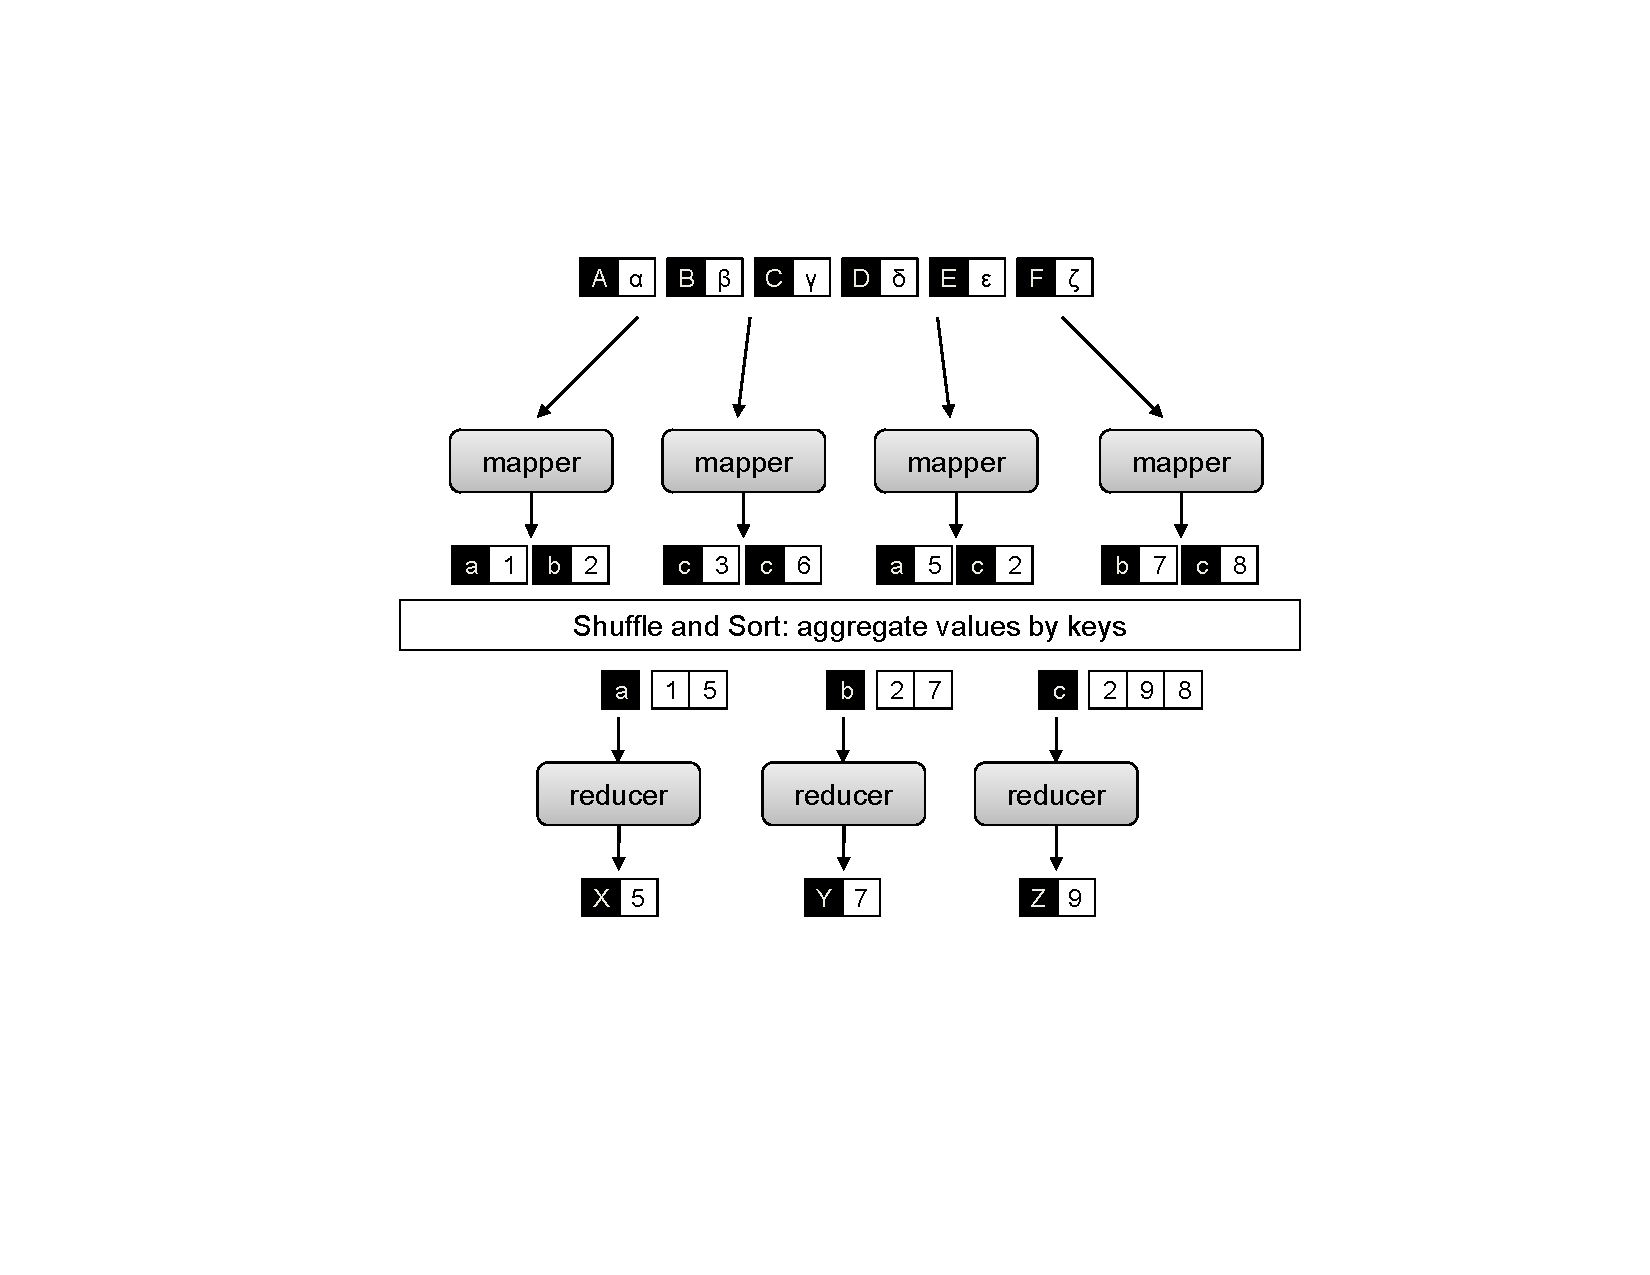
\includegraphics[scale=0.6]{figures/fig-ch2-MapReduce-simple.pdf}
\end{center}
\caption{Simplified view of MapReduce.  Mappers are applied to all
  input key-value pairs, which generate an arbitrary number of
  intermediate key-value pairs.  Reducers are applied to all values
  associated with the same key.  Between the map and reduce phases
  lies a barrier that involves a large distributed sort and group by.}
\label{figure:chapter2:MapReduce-simple}
\end{figure}

\begin{algorithm}[p]
\caption{Word count}
\label{algorithm:chapter2:word-count:basic}
The mapper emits an intermediate key-value pair for each word in a
document. The reducer sums up all counts for each word.
\algrenewcommand\algorithmicfunction{\textbf{class}}
\algrenewcommand\algorithmicprocedure{\textbf{method}}
  \begin{algorithmic}[1]
    \Function{Mapper}{}
    \Procedure{Map}{$\textrm{docid }a, \textrm{doc }d$}
    \ForAll{$\textrm{term }t \in \textrm{doc }d$}
    \State $\textsc{Emit}(\textrm{term }t, \textrm{count }1)$
    \EndFor
    \EndProcedure
    \EndFunction
  \end{algorithmic}

  \begin{algorithmic}[1]
    \Function{Reducer}{}
    \Procedure{Reduce}{$\textrm{term }t, \textrm{counts }[  c_1, c_2, \ldots ]$}
    \State $sum \gets 0$
    \ForAll{$ \textrm{count }c \in \textrm{counts }[  c_1, c_2, \ldots ]$}
    \State $sum \gets sum + c$
    \EndFor
    \State $\textsc{Emit}(\textrm{term }t, \textrm{count }sum)$
    \EndProcedure
    \EndFunction
  \end{algorithmic}
\end{algorithm}

A simple word count algorithm in MapReduce is shown in
Algorithm~\ref{algorithm:chapter2:word-count:basic}.  This algorithm counts the
number of occurrences of every word in a text collection, which may be
the first step in, for example, building a unigram language model
(i.e., probability distribution over words in a collection).  Input
key-values pairs take the form of (docid, doc) pairs stored on the
distributed file system, where the former is a unique identifier for
the document, and the latter is the text of the document itself.  The
mapper takes an input key-value pair, tokenizes the document, and
emits an intermediate key-value pair for every word:\ the word itself
serves as the key, and the integer one serves as the value (denoting
that we've seen the word once).  The MapReduce execution framework
guarantees that all values associated with the same key are brought
together in the reducer.  Therefore, in our word count algorithm, we
simply need to sum up all counts (ones) associated with each word.
The reducer does exactly this, and emits final key-value pairs with
the word as the key, and the count as the value.  Final output is
written to the distributed file system, one file per reducer.  Words
within each file will be sorted by alphabetical order, and each file
will contain roughly the same number of words.  The partitioner, which
we discuss later in Section~\ref{chapter2:partitioners-and-combiners},
controls the assignment of words to reducers.  The output can be
examined by the programmer or used as input to another MapReduce
program.

There are some differences between the Hadoop implementation of
MapReduce and Google's implementation.\footnote{Personal
communication, Jeff Dean.}  In Hadoop, the reducer is presented with a
key and an iterator over all values associated with the particular
key.  The values are arbitrarily ordered.  Google's implementation
allows the programmer to specify a secondary sort key for ordering the
values (if desired)---in which case values associated with each key
would be presented to the developer's reduce code in sorted order.
Later in Section~\ref{chapter3:secondary-sorting} we discuss how to
overcome this limitation in Hadoop to perform secondary sorting.
Another difference:\ in Google's implementation the programmer is not
allowed to change the key in the reducer.  That is, the reducer output
key must be exactly the same as the reducer input key.  In Hadoop,
there is no such restriction, and the reducer can emit an arbitrary
number of output key-value pairs (with different keys).

To provide a bit more implementation detail:\ pseudo-code provided in
this book roughly mirrors how MapReduce programs are written in
Hadoop.  Mappers and reducers are objects that implement
the \textsc{Map} and \textsc{Reduce} methods, respectively.  In
Hadoop, a mapper object is initialized for each map task (associated
with a particular sequence of key-value pairs called an input split)
and the \textsc{Map} method is called on each key-value pair by the
execution framework.  In configuring a MapReduce job, the programmer
provides a hint on the number of map tasks to run, but the execution
framework (see next section) makes the final determination based on
the physical layout of the data (more details in
Section~\ref{chapter2:dfs} and
Section~\ref{chapter2:cluster-architecture}).  The situation is
similar for the reduce phase:\ a reducer object is initialized for
each reduce task, and the \textsc{Reduce} method is called once per
intermediate key.  In contrast with the number of map tasks, the
programmer can precisely specify the number of reduce tasks.  We will
return to discuss the details of Hadoop job execution in
Section~\ref{chapter2:cluster-architecture}, which is dependent on an
understanding of the distributed file system (covered in
Section~\ref{chapter2:dfs}).  To reiterate:\ although the presentation
of algorithms in this book closely mirrors the way they would be
implemented in Hadoop, our focus is on algorithm design and conceptual
understanding---not actual Hadoop programming.  For that, we would
recommend Tom White's book~\cite{White_2009}.

What are the restrictions on mappers and reducers?  Mappers and
reducers can express arbitrary computations over their inputs.
However, one must generally be careful about use of external resources
since multiple mappers or reducers may be contending for those
resources.  For example, it may be unwise for a mapper to query an
external SQL database, since that would introduce a scalability
bottleneck on the number of map tasks that could be run in parallel
(since they might all be simultaneously querying the
database).\footnote{Unless, of course, the database itself is highly
scalable.} In general, mappers can emit an arbitrary number of
intermediate key-value pairs, and they need not be of the same type as
the input key-value pairs.  Similarly, reducers can emit an arbitrary
number of final key-value pairs, and they can differ in type from the
intermediate key-value pairs.  Although not permitted in functional
programming, mappers and reducers can have side effects.  This is a
powerful and useful feature:\ for example, preserving state across
multiple inputs is central to the design of many MapReduce algorithms
(see Chapter~\ref{chapter3}).  Such algorithms can be understood as
having side effects that only change state that is \emph{internal} to
the mapper or reducer.  While the correctness of such algorithms may
be more difficult to guarantee (since the function's behavior depends
not only on the current input but on previous inputs), most potential
synchronization problems are avoided since internal state is private
only to individual mappers and reducers.  In other cases (see
Section~\ref{chapter-indexing:index:revised} and
Section~\ref{chapter6_variants}), it may be useful for mappers or
reducers to have \emph{external} side effects, such as writing files
to the distributed file system.  Since many mappers and reducers are
run in parallel, and the distributed file system is a shared global
resource, special care must be taken to ensure that such operations
avoid synchronization conflicts.  One strategy is to write a temporary
file that is renamed upon successful completion of the mapper or
reducer~\cite{Dean_Ghemawat_OSDI2004}.

In addition to the ``canonical'' MapReduce processing flow, other
variations are also possible.  MapReduce programs can contain no
reducers, in which case mapper output is directly written to disk (one
file per mapper).  For embarrassingly parallel problems, e.g., parse a
large text collection or independently analyze a large number of
images, this would be a common pattern.  The converse---a MapReduce
program with no mappers---is not possible, although in some cases it
is useful for the mapper to implement the identity function and simply
pass input key-value pairs to the reducers.  This has the effect of
sorting and regrouping the input for reduce-side processing.
Similarly, in some cases it is useful for the reducer to implement the
identity function, in which case the program simply sorts and groups
mapper output.  Finally, running identity mappers and reducers has the
effect of regrouping and resorting the input data (which is sometimes
useful).

Although in the most common case, input to a MapReduce job comes from
data stored on the distributed file system and output is written back
to the distributed file system, any other system that satisfies the
proper abstractions can serve as a data source or sink.  With Google's
MapReduce implementation, BigTable~\cite{ChangFay_etal_OSDI2006}, a
sparse, distributed, persistent multidimensional sorted map, is
frequently used as a source of input and as a store of MapReduce
output.  HBase is an open-source BigTable clone and has similar
capabilities.  Also, Hadoop has been integrated with existing MPP
(massively parallel processing) relational databases, which allows a
programmer to write MapReduce jobs over database rows and dump output
into a new database table.  Finally, in some cases MapReduce jobs may
not consume any input at all (e.g., computing $\pi$) or may only
consume a small amount of data (e.g., input parameters to many
instances of processor-intensive simulations running in parallel).

\section{The Execution Framework}
\label{chapter2:execution-framework}

One of the most important idea behind MapReduce is separating the \emph{
what} of distributed processing from the \emph{how}.  A MapReduce
program, referred to as a job, consists of code for mappers and
reducers (as well as combiners and partitioners to be discussed in the
next section) packaged together with configuration parameters (such as
where the input lies and where the output should be stored).  The
developer submits the job to the submission node of a cluster (in
Hadoop, this is called the jobtracker) and execution framework
(sometimes called the ``runtime'') takes care of everything else:\ it
transparently handles all other aspects of distributed code execution,
on clusters ranging from a single node to a few thousand nodes.
Specific responsibilities include:

\paragraph{Scheduling.} Each MapReduce job is divided into smaller
units called tasks (see Section~\ref{chapter2:cluster-architecture}
for more details).  For example, a map task may be responsible for
processing a certain block of input key-value pairs (called an input
split in Hadoop); similarly, a reduce task may handle a portion of the
intermediate key space.  It is not uncommon for MapReduce jobs to have
thousands of individual tasks that need to be assigned to nodes in the
cluster.  In large jobs, the total number of tasks may exceed the
number of tasks that can be run on the cluster concurrently, making it
necessary for the scheduler to maintain some sort of a task queue and
to track the progress of running tasks so that waiting tasks can be
assigned to nodes as they become available.  Another aspect of
scheduling involves coordination among tasks belonging to different
jobs (e.g., from different users).  How can a large, shared resource
support several users simultaneously in a predictable, transparent,
policy-driven fashion?  There has been some recent work along these
lines in the context of
Hadoop~\cite{Sandholm_Lai_2009,Zaharia_etal_2009}.

Speculative execution is an optimization that is implemented by both
Hadoop and Google's MapReduce implementation (called ``backup
tasks''~\cite{Dean_Ghemawat_OSDI2004}).  Due to the barrier between
the map and reduce tasks, the map phase of a job is only as fast as
the slowest map task.  Similarly, the completion time of a job is
bounded by the running time of the slowest reduce task.  As a result,
the speed of a MapReduce job is sensitive to what are known as \emph{
stragglers}, or tasks that take an usually long time to complete.  One
cause of stragglers is flaky hardware:\ for example, a machine that is
suffering from recoverable errors may become significantly slower.
With speculative execution, an identical copy of the same task is
executed on a different machine, and the framework simply uses the
result of the first task attempt to finish.  Zaharia et
al.~\cite{Zaharia_etal_OSDI2008} presented different execution
strategies in a recent paper, and Google has reported that speculative
execution can improve job running times by
44\%~\cite{Dean_Ghemawat_OSDI2004}.  Although in Hadoop both map and
reduce tasks can be speculatively executed, the common wisdom is that
the technique is more helpful for map tasks than reduce tasks, since
each copy of the reduce task needs to pull data over the network.
Note, however, that speculative execution cannot adequately address
another common cause of stragglers:\ skew in the distribution of
values associated with intermediate keys (leading to reduce
stragglers).  In text processing we often observe Zipfian
distributions, which means that the task or tasks responsible for
processing the most frequent few elements will run much longer than
the typical task.  Better local aggregation, discussed in the next
chapter, is one possible solution to this problem.

\paragraph{Data/code co-location.}  The phrase \emph{data
  distribution} is misleading, since one of the key ideas behind
MapReduce is to move the code, not the data.  However, the more
general point remains---in order for computation to occur, we need to
somehow feed data to the code.  In MapReduce, this issue is
inextricably intertwined with scheduling and relies heavily on the
design of the underlying distributed file system.\footnote{In the
canonical case, that is.  Recall that MapReduce may receive its input
from other sources.} To achieve data locality, the scheduler starts
tasks on the node that holds a particular block of data (i.e., on its
local drive) needed by the task.  This has the effect of moving code
to the data.  If this is not possible (e.g., a node is already running
too many tasks), new tasks will be started elsewhere, and the
necessary data will be streamed over the network.  An important
optimization here is to prefer nodes that are on the same rack in the
datacenter as the node holding the relevant data block, since
inter-rack bandwidth is significantly less than intra-rack bandwidth.

\paragraph{Synchronization.} In general, synchronization refers to
the mechanisms by which multiple concurrently running processes ``join
up'', for example, to share intermediate results or otherwise exchange
state information.  In MapReduce, synchronization is accomplished by a
barrier between the map and reduce phases of processing.  Intermediate
key-value pairs must be grouped by key, which is accomplished by a
large distributed sort involving all the nodes that executed map tasks
and all the nodes that will execute reduce tasks.  This necessarily
involves copying intermediate data over the network, and therefore the
process is commonly known as ``shuffle and sort''.  A MapReduce job
with $m$ mappers and $r$ reducers involves up to $m \times r$ distinct
copy operations, since each mapper may have intermediate output going
to every reducer.

Note that the reduce computation cannot start until all the mappers
have finished emitting key-value pairs and all intermediate key-value
pairs have been shuffled and sorted, since the execution framework
cannot otherwise guarantee that all values associated with the same
key have been gathered.  This is an important departure from
functional programming:\ in a \emph{fold} operation, the aggregation
function $g$ is a function of the intermediate value and the next item
in the list---which means that values can be lazily generated and
aggregation can begin as soon as values are available.  In contrast,
the reducer in MapReduce receives \emph{all} values associated with the
same key at once.  However, it is possible to start copying
intermediate key-value pairs over the network to the nodes running the
reducers as soon as each mapper finishes---this is a common
optimization and implemented in Hadoop.

\paragraph{Error and fault handling.}  The MapReduce execution
framework must accomplish all the tasks above in an environment where
errors and faults are the norm, not the exception.  Since MapReduce
was explicitly designed around low-end commodity servers, the runtime
must be especially resilient.  In large clusters, disk failures are
common~\cite{Pinheiro_etal_2007} and RAM experiences more errors than
one might expect~\cite{Schroeder_etal_2009}.  Datacenters suffer from
both planned outages (e.g., system maintenance and hardware upgrades)
and unexpected outages (e.g., power failure, connectivity loss, etc.).

And that's just hardware.  No software is bug free---exceptions must
be appropriately trapped, logged, and recovered from.  Large-data
problems have a penchant for uncovering obscure corner cases in code
that is otherwise thought to be bug-free.  Furthermore, any
sufficiently large dataset will contain corrupted data or records that
are mangled beyond a programmer's imagination---resulting in errors
that one would never think to check for or trap.  The MapReduce
execution framework must thrive in this hostile environment.

\section{Partitioners and Combiners}
\label{chapter2:partitioners-and-combiners}

We have thus far presented a simplified view of MapReduce.  There are
two additional elements that complete the programming model:\
partitioners and combiners.

Partitioners are responsible for dividing up the intermediate key
space and assigning intermediate key-value pairs to reducers.  In
other words, the partitioner specifies the task to which an
intermediate key-value pair must be copied.  Within each reducer, keys
are processed in sorted order (which is how the ``group by'' is
implemented).  The simplest partitioner involves computing the hash
value of the key and then taking the mod of that value with the number
of reducers.  This assigns approximately the same number of keys to
each reducer (dependent on the quality of the hash function).  Note,
however, that the partitioner only considers the key and ignores the
value---therefore, a roughly-even partitioning of the key space may
nevertheless yield large differences in the number of key-values pairs
sent to each reducer (since different keys may have different numbers
of associated values).  This imbalance in the amount of data
associated with each key is relatively common in many text processing
applications due to the Zipfian distribution of word occurrences.

Combiners are an optimization in MapReduce that allow for local
aggregation before the shuffle and sort phase.  We can motivate the
need for combiners by considering the word count algorithm in
Algorithm~\ref{algorithm:chapter2:word-count:basic}, which emits a key-value pair
for each word in the collection.  Furthermore, all these key-value
pairs need to be copied across the network, and so the amount of
intermediate data will be larger than the input collection itself.
This is clearly inefficient.  One solution is to perform local
aggregation on the output of each mapper, i.e., to compute a local
count for a word over all the documents processed by the mapper.  With
this modification (assuming the maximum amount of local aggregation
possible), the number of intermediate key-value pairs will be at most
the number of unique words in the collection times the number of
mappers (and typically far smaller because each mapper may not
encounter every word).

The combiner in MapReduce supports such an optimization.  One can
think of combiners as ``mini-reducers'' that take place on the output
of the mappers, prior to the shuffle and sort phase.  Each combiner
operates in isolation and therefore does not have access to
intermediate output from other mappers.  The combiner is provided keys
and values associated with each key (the same types as the mapper
output keys and values).  Critically, one cannot assume that a
combiner will have the opportunity to process \emph{all} values
associated with the same key.  The combiner can emit any number of
key-value pairs, but the keys and values must be of the same type as
the mapper output (same as the reducer input).\footnote{A note on the
implementation of combiners in Hadoop:\ by default, the execution
framework reserves the right to use combiners at its discretion.  In
reality, this means that a combiner may be invoked zero, one, or
multiple times.  In addition, combiners in Hadoop may actually be
invoked in the reduce phase, i.e., after key-value pairs have been
copied over to the reducer, but before the user reducer code runs.  As
a result, combiners must be carefully written so that they can be
executed in these different environments.
Section~\ref{chapter3:local-aggregation:correctness} discusses this in
more detail.}  In cases where an operation is both associative and
commutative (e.g., addition or multiplication), reducers can directly
serve as combiners.  In general, however, reducers and combiners are
not interchangeable.

In many cases, proper use of combiners can spell the difference
between an impractical algorithm and an efficient algorithm.  This
topic will be discussed in Section~\ref{chapter3:local-aggregation},
which focuses on various techniques for local aggregation.  It
suffices to say for now that a combiner can significantly reduce the
amount of data that needs to be copied over the network, resulting in
much faster algorithms.

The complete MapReduce model is shown in
Figure~\ref{figure:chapter2:MapReduce-complete}.  Output of the
mappers are processed by the combiners, which perform local
aggregation to cut down on the number of intermediate key-value pairs.
The partitioner determines which reducer will be responsible for
processing a particular key, and the execution framework uses this
information to copy the data to the right location during the shuffle
and sort phase.\footnote{In Hadoop, partitioners are actually executed
before combiners, so while
Figure~\ref{figure:chapter2:MapReduce-complete} is conceptually
accurate, it doesn't precisely describe the Hadoop implementation.}
Therefore, a complete MapReduce job consists of code for the mapper,
reducer, combiner, and partitioner, along with job configuration
parameters.  The execution framework handles everything else.

\begin{figure}[t]
\begin{center}
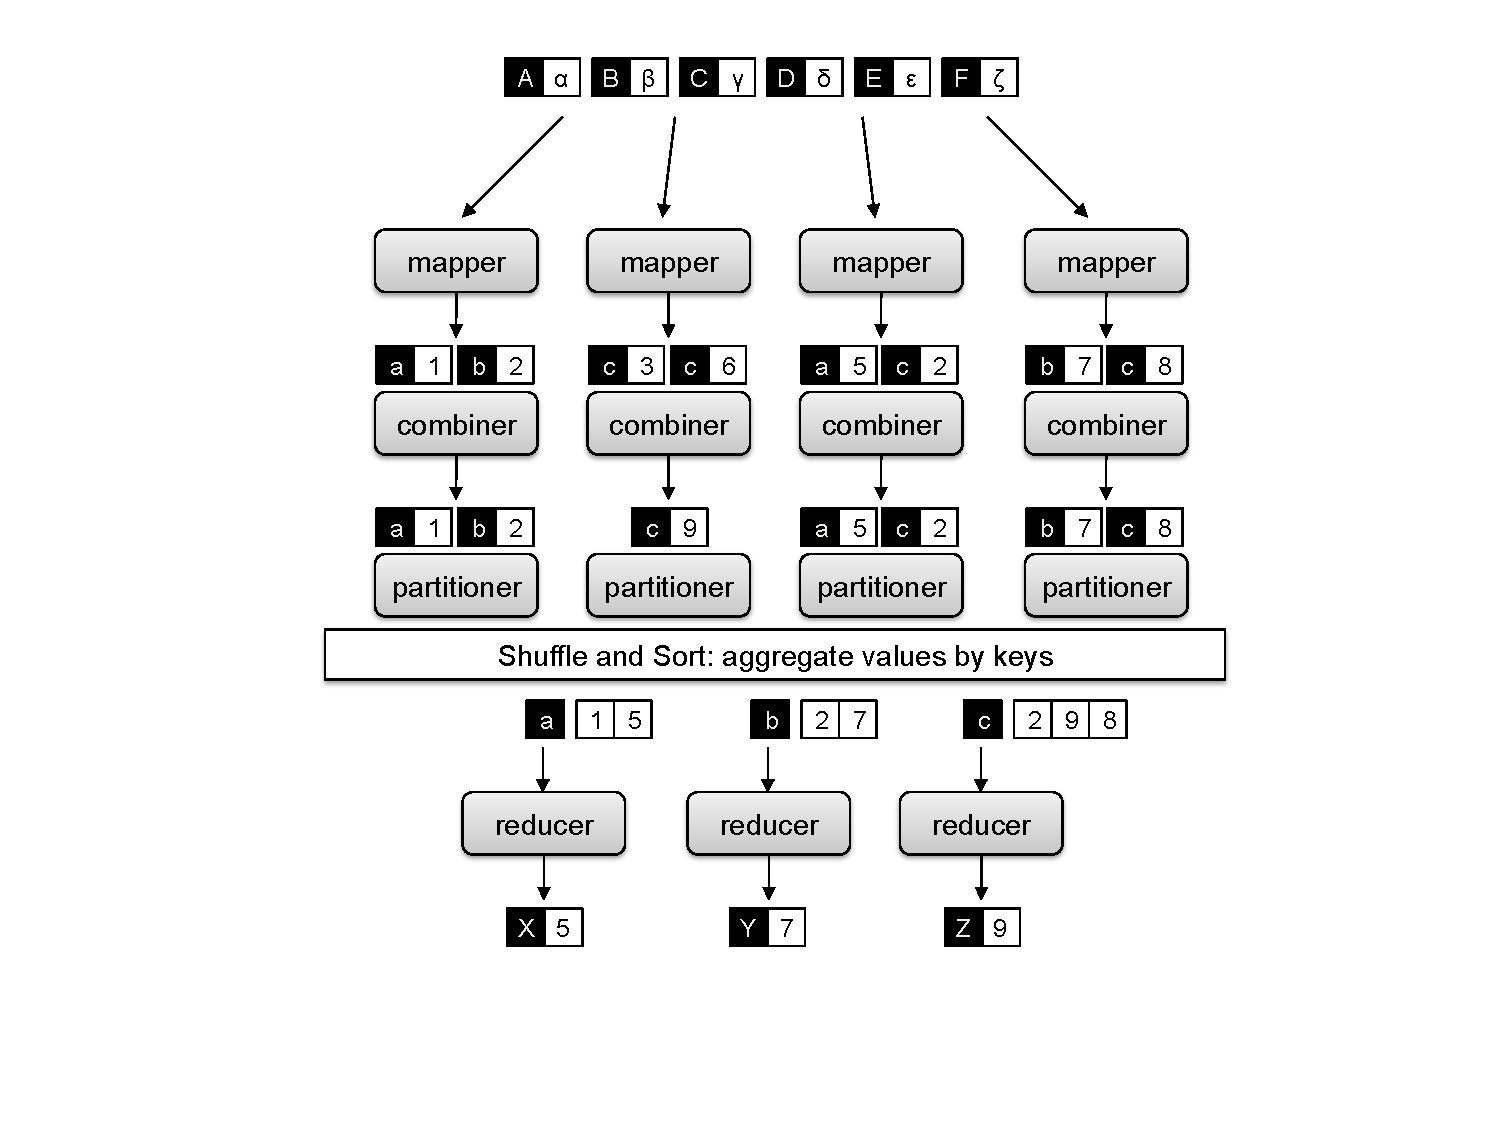
\includegraphics[scale=0.6]{figures/fig-ch2-MapReduce-complete.pdf}
\end{center}
\caption{Complete view of MapReduce, illustrating combiners and
  partitioners in addition to mappers and reducers.  Combiners can be
  viewed as ``mini-reducers'' in the map phase.  Partitioners
  determine which reducer is responsible for a particular key.}
\label{figure:chapter2:MapReduce-complete}
\end{figure}

\section{The Distributed File System}
\label{chapter2:dfs}

So far, we have mostly focused on the \emph{processing} aspect of
data-intensive processing, but it is important to recognize that
without data, there is nothing to compute on.  In high-performance
computing (HPC) and many traditional cluster architectures, storage is
viewed as a distinct and separate component from computation.
Implementations vary widely, but network-attached storage (NAS) and
storage area networks (SAN) are common; supercomputers often have
dedicated subsystems for handling storage (separate nodes, and often
even separate networks).  Regardless of the details, the processing
cycle remains the same at a high level:\ the compute nodes fetch input
from storage, load the data into memory, process the data, and then
write back the results (with perhaps intermediate checkpointing for
long-running processes).

As dataset sizes increase, more compute capacity is required for
processing.  But as compute capacity grows, the link between the
compute nodes and the storage becomes a bottleneck.  At that point,
one could invest in higher performance but more expensive networks
(e.g., 10 gigabit Ethernet) or special-purpose interconnects such as
InfiniBand (even more expensive).  In most cases, this is not a
cost-effective solution, as the price of networking equipment
increases non-linearly with performance (e.g., a switch with ten times
the capacity is usually more than ten times more expensive).
Alternatively, one could abandon the separation of computation and
storage as distinct components in a cluster.  The distributed file
system (DFS) that underlies MapReduce adopts exactly this approach.
The Google File System (GFS)~\cite{Ghemawat_etal_SOSP2003} supports
Google's proprietary implementation of MapReduce; in the open-source
world, HDFS (Hadoop Distributed File System) is an open-source
implementation of GFS that supports Hadoop.  Although MapReduce
doesn't necessarily require the distributed file system, it is
difficult to realize many of the advantages of the programming model
without a storage substrate that behaves much like the
DFS.\footnote{However, there is evidence that existing POSIX-based
distributed cluster file systems (e.g., GPFS or PVFS) can serve as a
replacement for HDFS, when properly tuned or modified for MapReduce
workloads~\cite{Tantisiriroj_etal_2008,Ananthanarayanan_etal_2009}.
This, however, remains an experimental use case.}

Of course, distributed file systems are not
new~\cite{Howard_etal_1988,Cabrera_Long_1991,Anderson_etal_SOSP1995,Thekkath_etal_SOSP1997,Schmuck_Haskin_2002}.
The MapReduce distributed file system builds on previous work but is
specifically adapted to large-data processing workloads, and therefore
departs from previous architectures in certain respects (see
discussion by Ghemawat et al.~\cite{Ghemawat_etal_SOSP2003} in the
original GFS paper.).  The main idea is to divide user data into
blocks and replicate those blocks across the local disks of nodes in
the cluster.  Blocking data, of course, is not a new idea, but DFS
blocks are significantly larger than block sizes in typical
single-machine file systems (64 MB by default).  The distributed file
system adopts a master--slave architecture in which the master
maintains the file namespace (metadata, directory structure, file to
block mapping, location of blocks, and access permissions) and the
slaves manage the actual data blocks.  In GFS, the master is called
the GFS master, and the slaves are called GFS chunkservers.  In
Hadoop, the same roles are filled by the namenode and datanodes,
respectively.\footnote{To be precise, namenode and datanode may refer
to physical machines in a cluster, or they may refer to daemons
running on those machines providing the relevant services.} This book
adopts the Hadoop terminology, although for most basic file operations
GFS and HDFS work much the same way.  The architecture of HDFS is
shown in Figure~\ref{figure:chapter2:HDFS}, redrawn from a similar
diagram describing GFS~\cite{Ghemawat_etal_SOSP2003}.

\begin{figure}[t]
\begin{center}
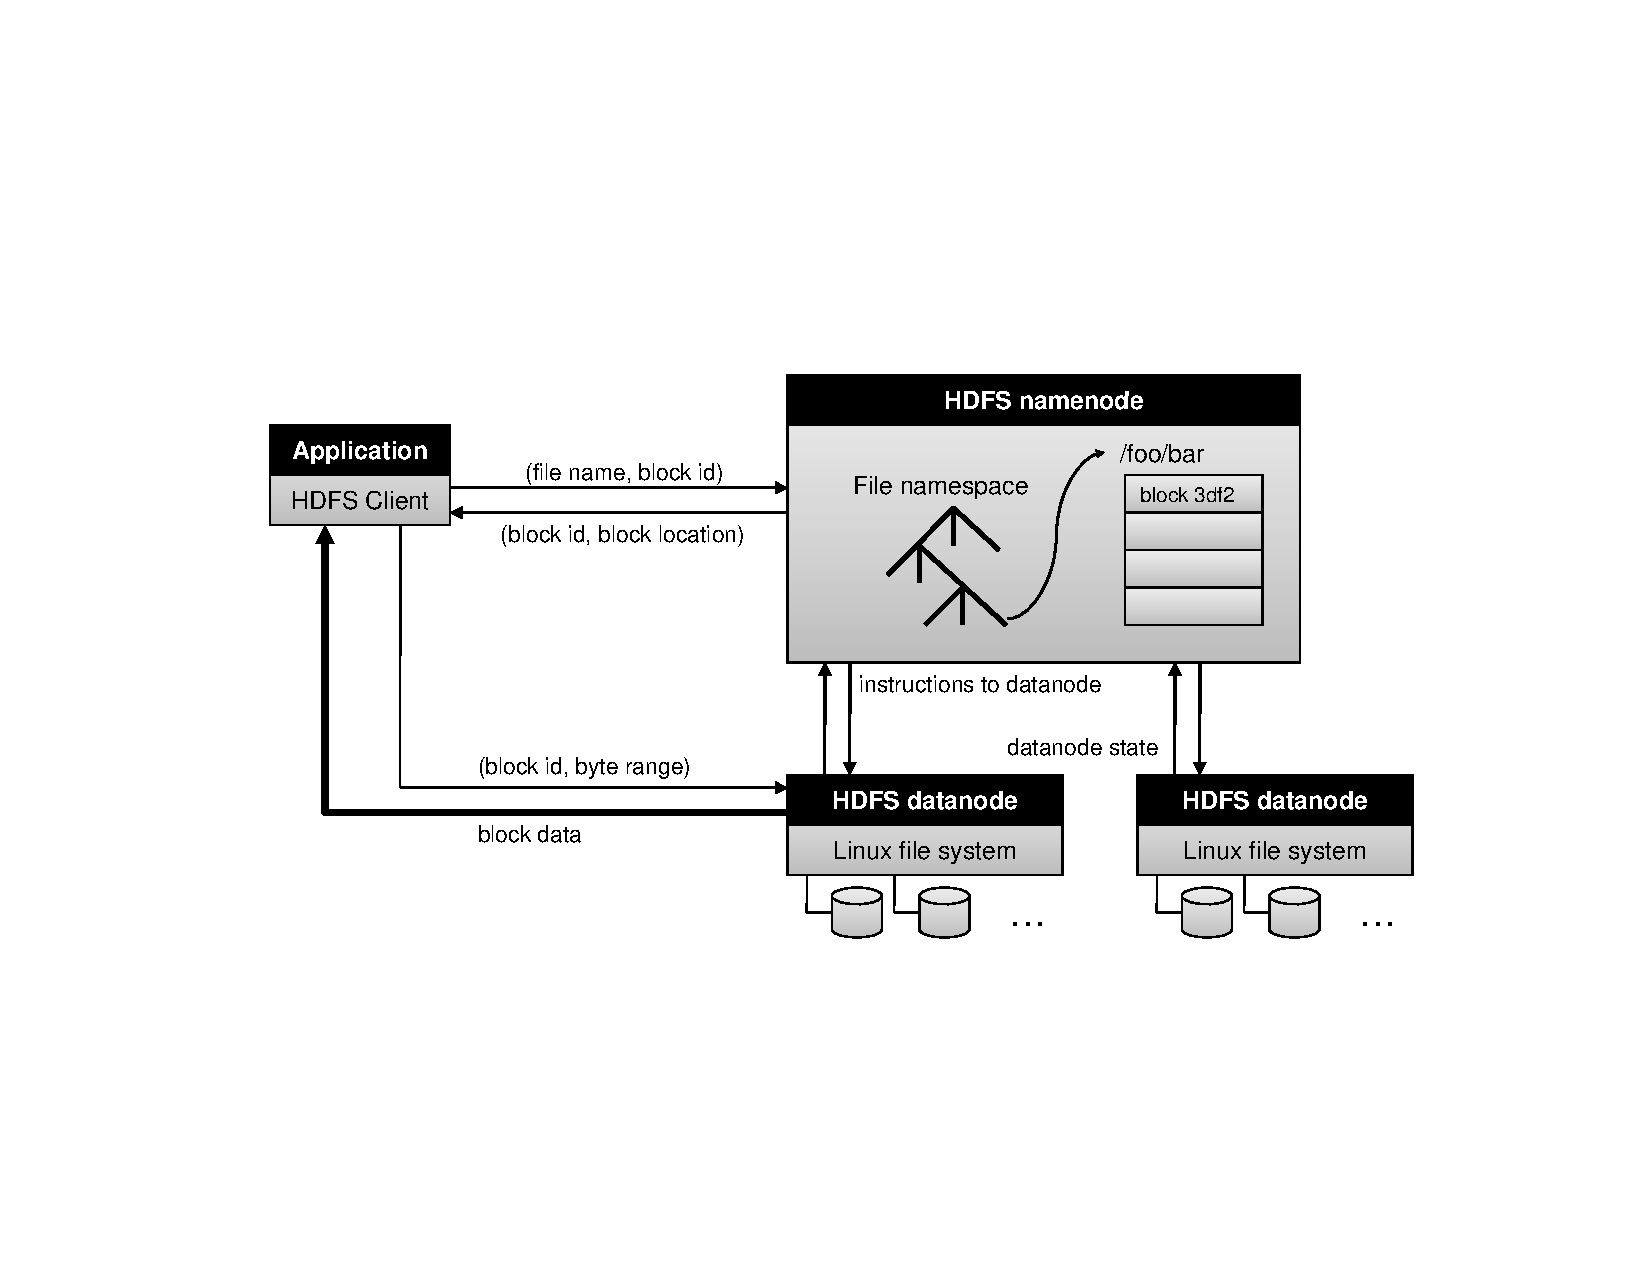
\includegraphics[scale=0.6]{figures/fig-ch2-HDFS.pdf}
\end{center}
\caption{The architecture of HDFS.  The namenode (master) is responsible for maintaining the file
  namespace and directing clients to datanodes (slaves) that actually
  hold data blocks containing user data.}
\label{figure:chapter2:HDFS}
\end{figure}

In HDFS, an application client wishing to read a file (or a portion
thereof) must first contact the namenode to determine where the actual
data is stored.  In response to the client request, the namenode
returns the relevant block id and the location where the block is held
(i.e., which datanode).  The client then contacts the datanode to
retrieve the data.  Blocks are themselves stored on standard
single-machine file systems, so HDFS lies on top of the standard OS
stack (e.g., Linux).  An important feature of the design is that data
is never moved through the namenode.  Instead, all data transfer
occurs directly between clients and datanodes; communications with the
namenode only involves transfer of metadata.

By default, HDFS stores three separate copies of each data block to
ensure both reliability, availability, and performance.  In large
clusters, the three replicas are spread across different physical
racks, so HDFS is resilient towards two common failure scenarios:\
individual datanode crashes and failures in networking equipment that
bring an entire rack offline.  Replicating blocks across physical
machines also increases opportunities to co-locate data and processing
in the scheduling of MapReduce jobs, since multiple copies yield more
opportunities to exploit locality.  The namenode is in periodic
communication with the datanodes to ensure proper replication of all
the blocks:\ if there aren't enough replicas (e.g., due to disk or
machine failures or to connectivity losses due to networking equipment
failures), the namenode directs the creation of additional
copies;\footnote{Note that the namenode coordinates the replication
process, but data transfer occurs directly from datanode to datanode.}
if there are too many replicas (e.g., a repaired node rejoins the
cluster), extra copies are discarded.

To create a new file and write data to HDFS, the application client
first contacts the namenode, which updates the file namespace after
checking permissions and making sure the file doesn't already exist.
The namenode allocates a new block on a suitable datanode, and the
application is directed to stream data directly to it.  From the
initial datanode, data is further propagated to additional replicas.
In the most recent release of Hadoop as of this writing (release
0.20.2), files are immutable---they cannot be modified after creation.
There are current plans to officially support file appends in the near
future, which is a feature already present in GFS.

In summary, the HDFS namenode has the following responsibilities:

\begin{itemize}

\item Namespace management.  The namenode is responsible for
  maintaining the file namespace, which includes metadata, directory
  structure, file to block mapping, location of blocks, and access
  permissions.  These data are held in memory for fast access and all
  mutations are persistently logged.

\item Coordinating file operations.  The namenode directs application
  clients to datanodes for read operations, and allocates blocks on
  suitable datanodes for write operations.  All data transfers occur
  directly between clients and datanodes.  When a file is deleted,
  HDFS does not immediately reclaim the available physical storage;
  rather, blocks are lazily garbage collected.

\item Maintaining overall health of the file system. The namenode is
  in periodic contact with the datanodes via heartbeat messages to
  ensure the integrity of the system.  If the namenode observes that a
  data block is under-replicated (fewer copies are stored on datanodes
  than the desired replication factor), it will direct the creation of
  new replicas.  Finally, the namenode is also responsible for
  rebalancing the file system.\footnote{In Hadoop, this is a
  manually-invoked process.}  During the course of normal operations,
  certain datanodes may end up holding more blocks than others;
  rebalancing involves moving blocks from datanodes with more blocks
  to datanodes with fewer blocks.  This leads to better load balancing
  and more even disk utilization.

\end{itemize}

\noindent Since GFS and HDFS were specifically designed to support
Google's proprietary and the open-source implementation of MapReduce,
respectively, they were designed with a number of assumptions about
the operational environment, which in turn influenced the design of
the systems.  Understanding these choices is critical to designing
effective MapReduce algorithms:

\begin{itemize}

\item The file system stores a relatively modest number of large
  files.  The definition of ``modest'' varies by the size of the
  deployment, but in HDFS multi-gigabyte files are common (and even
  encouraged).  There are several reasons why lots of small files are
  to be avoided.  Since the namenode must hold all file metadata in
  memory, this presents an upper bound on both the number of files and
  blocks that can be supported.\footnote{According to Dhruba Borthakur
  in a post to the Hadoop mailing list on 6/8/2008, each block in HDFS
  occupies about 150 bytes of memory on the namenode.} Large
  multi-block files represent a more efficient use of namenode memory
  than many single-block files (each of which consumes less space than
  a single block size).  In addition, mappers in a MapReduce job use
  individual files as a basic unit for splitting input data.  At
  present, there is no default mechanism in Hadoop that allows a
  mapper to process multiple files.  As a result, mapping over many
  small files will yield as many map tasks as there are files.  This
  results in two potential problems:\ first, the startup costs of
  mappers may become significant compared to the time spent actually
  processing input key-value pairs; second, this may result in an
  excessive amount of across-the-network copy operations during the
  ``shuffle and sort'' phase (recall that a MapReduce job with $m$
  mappers and $r$ reducers involves up to $m \times r$ distinct copy
  operations).

\item Workloads are batch oriented, dominated by long streaming
  reads and large sequential writes.  As a result, high sustained
  bandwidth is more important than low latency.  This exactly
  describes the nature of MapReduce jobs, which are batch operations
  on large amounts of data.  Due to the common-case workload, both
  HDFS and GFS do not implement any form of data
  caching.\footnote{However, since the distributed file system is
  built on top of a standard operating system such as Linux, there is
  still OS-level caching.}

\item Applications are aware of the characteristics of the distributed
  file system.  Neither HDFS nor GFS present a general POSIX-compliant
  API, but rather support only a subset of possible file operations.
  This simplifies the design of the distributed file system, and in
  essence pushes part of the data management onto the end application.
  One rationale for this decision is that each application knows best
  how to handle data specific to that application, for example, in
  terms of resolving inconsistent states and optimizing the layout of
  data structures.

\item The file system is deployed in an environment of cooperative
  users.  There is no discussion of security in the original GFS
  paper, but HDFS explicitly assumes a datacenter environment where
  only authorized users have access.  File permissions in HDFS are
  only meant to prevent unintended operations and can be easily
  circumvented.\footnote{However, there are existing plans to
  integrate Kerberos into Hadoop/HDFS.}

\item The system is built from unreliable but inexpensive commodity
  components.  As a result, failures are the norm rather than the
  exception.  HDFS is designed around a number of self-monitoring and
  self-healing mechanisms to robustly cope with common failure modes.

\end{itemize}

\noindent Finally, some discussion is necessary to understand the
single-master design of HDFS and GFS.  It has been demonstrated that
in large-scale distributed systems, simultaneously providing
consistency, availability, and partition tolerance is
impossible---this is Brewer's so-called CAP
Theorem~\cite{Gilbert_Lynch_2002}.  Since partitioning is unavoidable
in large-data systems, the real tradeoff is between consistency and
availability.  A single-master design trades availability for
consistency and significantly simplifies implementation.  If the
master (HDFS namenode or GFS master) goes down, the entire file system
becomes unavailable, which trivially guarantees that the file system
will never be in an inconsistent state.  An alternative design might
involve multiple masters that jointly manage the file namespace---such
an architecture would increase availability (if one goes down, another
can step in) at the cost of consistency, not to mention requiring a
more complex implementation
(cf.~\cite{Alvaro_etal_2009,McKusick_Quinlan_2009}).

The single-master design of GFS and HDFS is a well-known weakness,
since if the master goes offline, the entire file system and all
MapReduce jobs running on top of it will grind to a halt.  This
weakness is mitigated in part by the lightweight nature of file system
operations.  Recall that no data is ever moved through the namenode
and that all communication between clients and datanodes involve only
metadata.  Because of this, the namenode rarely is the bottleneck, and
for the most part avoids load-induced crashes.  In practice, this
single point of failure is not as severe a limitation as it may
appear---with diligent monitoring of the namenode, mean time between
failure measured in months are not uncommon for production
deployments.  Furthermore, the Hadoop community is well-aware of this
problem and has developed several reasonable workarounds---for
example, a warm standby namenode that can be quickly switched over
when the primary namenode fails.  The open source environment and the
fact that many organizations already depend on Hadoop for production
systems virtually guarantees that more effective solutions will be
developed over time.

\section{Hadoop Cluster Architecture}
\label{chapter2:cluster-architecture}

Putting everything together, the architecture of a complete Hadoop
cluster is shown in Figure~\ref{figure:chapter2:Hadoop-cluster}.  The
HDFS namenode runs the namenode daemon.  The job submission node runs
the jobtracker, which is the single point of contact for a client
wishing to execute a MapReduce job.  The jobtracker monitors the
progress of running MapReduce jobs and is responsible for coordinating
the execution of the mappers and reducers.  Typically, these services
run on two separate machines, although in smaller clusters they are
often co-located.  The bulk of a Hadoop cluster consists of slave
nodes (only three of which are shown in the figure) that run both a
tasktracker, which is responsible for actually running user code, and
a datanode daemon, for serving HDFS data.

\begin{figure}[t]
\begin{center}
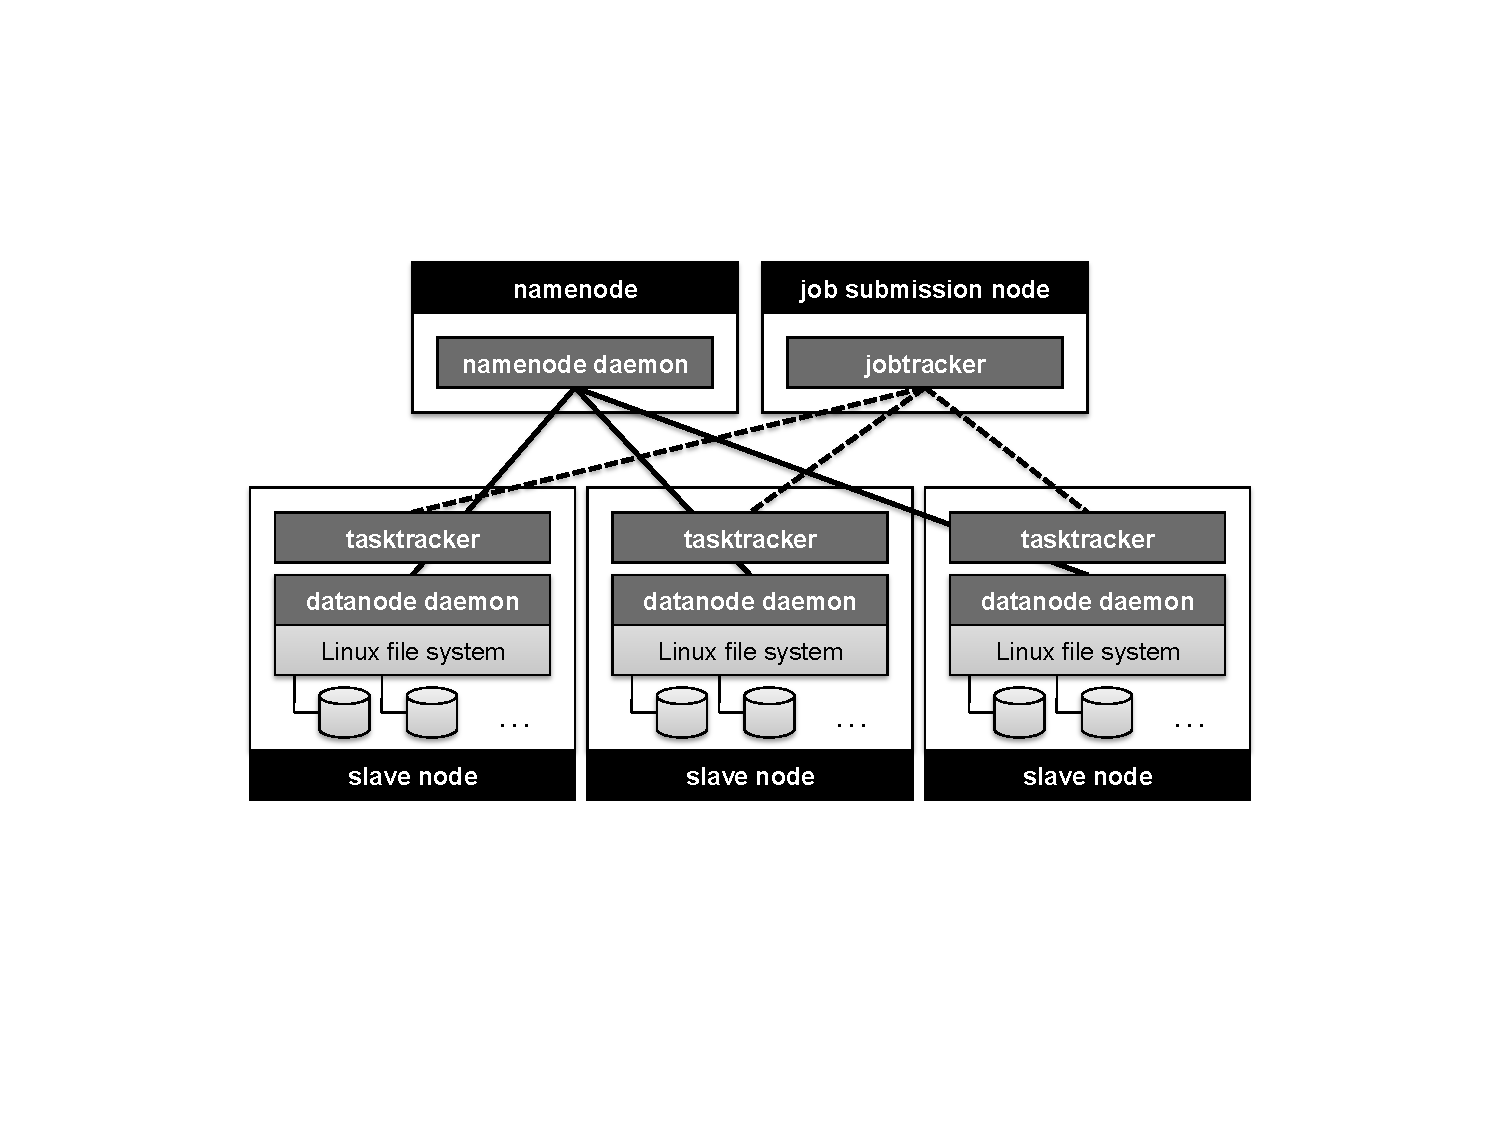
\includegraphics[scale=0.6]{figures/fig-ch2-Hadoop.pdf}
\end{center}
\caption{Architecture of a complete Hadoop cluster, which consists of
  three separate components:\ the HDFS master (called the namenode),
  the job submission node (called the jobtracker), and many slave
  nodes (three shown here).  Each of the slave nodes runs a
  tasktracker for executing map and reduce tasks and a datanode daemon
  for serving HDFS data.}
\label{figure:chapter2:Hadoop-cluster}
\end{figure}

A Hadoop MapReduce job is divided up into a number of map tasks and
reduce tasks.  Tasktrackers periodically send heartbeat messages to
the jobtracker that also doubles as a vehicle for task allocation.  If
a tasktracker is available to run tasks (in Hadoop parlance, has empty
task slots), the return acknowledgment of the tasktracker heartbeat
contains task allocation information.  The number of reduce tasks is
equal to the number of reducers specified by the programmer.  The
number of map tasks, on the other hand, depends on many factors:\ the
number of mappers specified by the programmer serves as a hint to the
execution framework, but the actual number of tasks depends on both
the number of input files and the number of HDFS data blocks occupied
by those files.  Each map task is assigned a sequence of input
key-value pairs, called an input split in Hadoop.  Input splits are
computed automatically and the execution framework strives to align
them to HDFS block boundaries so that each map task is associated with
a single data block.  In scheduling map tasks, the jobtracker tries to
take advantage of data locality---if possible, map tasks are scheduled
on the slave node that holds the input split, so that the mapper will
be processing local data.  The alignment of input splits with HDFS
block boundaries simplifies task scheduling.  If it is not possible to
run a map task on local data, it becomes necessary to stream input
key-value pairs across the network.  Since large clusters are
organized into racks, with far greater intra-rack bandwidth than
inter-rack bandwidth, the execution framework strives to at least
place map tasks on a rack which has a copy of the data block.

Although conceptually in MapReduce one can think of the mapper being
applied to all input key-value pairs and the reducer being applied to
all values associated with the same key, actual job execution is a bit
more complex.  In Hadoop, mappers are Java objects with a \textsc{Map}
method (among others).  A mapper object is instantiated for every map
task by the tasktracker.  The life-cycle of this object begins with
instantiation, where a hook is provided in the API to run
programmer-specified code.  This means that mappers can read in ``side
data'', providing an opportunity to load state, static data sources,
dictionaries, etc.  After initialization, the \textsc{Map} method is
called (by the execution framework) on all key-value pairs in the
input split.  Since these method calls occur in the context of the
same Java object, it is possible to preserve state across multiple
input key-value pairs within the same map task---this is an important
property to exploit in the design of MapReduce algorithms, as we will
see in the next chapter.  After all key-value pairs in the input split
have been processed, the mapper object provides an opportunity to run
programmer-specified termination code.  This, too, will be important
in the design of MapReduce algorithms.

The actual execution of reducers is similar to that of the mappers.
Each reducer object is instantiated for every reduce task.  The Hadoop
API provides hooks for programmer-specified initialization and
termination code.  After initialization, for each intermediate key in
the partition (defined by the partitioner), the execution framework
repeatedly calls the \textsc{Reduce} method with an intermediate key
and an iterator over all values associated with that key.  The
programming model also guarantees that intermediate keys will be
presented to the \textsc{Reduce} method in sorted order.  Since this
occurs in the context of a single object, it is possible to preserve
state across multiple intermediate keys (and associated values) within
a single reduce task.  Once again, this property is critical in the
design of MapReduce algorithms and will be discussed in the next
chapter.

\section{Summary}
\label{chapter2:summary}

This chapter provides a basic overview of the MapReduce programming
model, starting with its roots in functional programming and
continuing with a description of mappers, reducers, partitioners, and
combiners.  Significant attention is also given to the underlying
distributed file system, which is a tightly-integrated component of
the MapReduce environment.  Given this basic understanding, we now
turn our attention to the design of MapReduce algorithms.
